\documentclass[a4paper, 11pt]{article}

\usepackage{fullpage}

\usepackage[english,russian]{babel}
\usepackage[utf8]{inputenc}
\usepackage{amsmath, amsfonts, amssymb, amsthm}
\usepackage{mathtools}
\usepackage{bm}

\usepackage{hyperref}
\usepackage{booktabs}
\usepackage{graphicx}
\usepackage{subcaption}

\usepackage[linesnumbered,ruled,vlined]{algorithm2e}
\SetKwInput{KwInput}{input}
\SetAlFnt{\small}

\usepackage{float}

\newtheorem{definition}{Определение}
\newtheorem{theorem}{Теорема}
\newtheorem{lemma}{Лемма}

\begin{document}

\begin{titlepage}
	\newpage
	
	\begin{center}
		%	Московский Государственный Университет им. М. В. Ломоносова \\
	\end{center}
	
	\vspace{8em}
	
	\begin{center}
		%\Large Кафедра Вычислительных Технологий и Моделирования \\ 
	\end{center}
	
	\vspace{2em}
	
	\begin{center}
		\textsc{\textbf{Метод конечных элементов: теоретические сведения и программная реализация}}
	\end{center}
	
	\vspace{6em}
	
	
	
	\newbox{\lbox}
	\savebox{\lbox}{\hbox{}}
	\newlength{\maxl}
	\setlength{\maxl}{\wd\lbox}
	\hfill\parbox{11cm}{
		%\hspace*{5cm}\hspace*{-5cm}Студент:\hfill\hbox {Иванов И. И.\hfill}\\
		%\hspace*{5cm}\hspace*{-5cm}Преподаватель:\hfill\hbox {Ануприенко Д. В.\hfill}\\
		%	\\
		%\hspace*{5cm}\hspace*{-5cm}Группа:\hfill\hbox {403}\\
	}
	
	
	\vspace{\fill}
	
	\begin{center}
		Москва \\ 2022
	\end{center}
	
\end{titlepage}

\setcounter{MaxMatrixCols}{20}


\section{Метод Ритца поиска приближенных обобщенных решений операторных уравнений}
Метод Ритца -- вариационный и проекционный метод, с помощью которого можно приближенно находить обобщенные решения операторных уравнений в гильбертовых пространствах. Далее мы еще поясним, что это такое. Этот метод появился на рубеже XIX--XX веков и первоначально применялся инженерами для решения задач механики твердого тела. Похожими методами являются метод Бубнова--Галёркина, Галёркина--Петрова. Далее приводится проекционная форма метода Ритца.

Рассмотрим следующее операторное уравнение:
\begin{equation}\label{eq:ritz_op_eq}
\mathcal{A}u = f,~~~\mathcal{A}: H \rightarrow H,
\end{equation}
где $f \in H$, а $\mathcal{A}$ -- некоторый оператор, действующий в гильбертом пространстве $H$. Он имеет следующие свойства:
\begin{itemize}
	\item Область его определения $D(\mathcal{A})$ плотна в $H$, т.е. $\overline{D(\mathcal{A})} = H$;
	\item $\mathcal{A}$ -- симметричный, т.е. $(\mathcal{A}u,v) = (u,\mathcal{A}v)~~\forall u,v \in D(\mathcal{A})$;
	\item $\mathcal{A}$ -- положительно определённый, т.е. $\exists \gamma: (\mathcal{A}u,u) \ge \gamma^2 ||u||^2~~\forall u \in D(\mathcal{A})$.
\end{itemize}

Пользуясь этими свойствами, на $D(\mathcal{A})$ можно ввести новое скалярное произведение $[u,v] = (\mathcal{A}u,v)$ и порождаемую им \textit{энергетическую норму} $[u] = \sqrt{(Au,u)}$, а с её помощью ввести специальное
\textit{энергетическое пространство} $H_\mathcal{A}$ -- пополнение $D(\mathcal{A})$ по энергетической норме. 

Введя энергетическое пространство, можно рассматривать так называемую \textit{слабую постановку задачи}. Это понятие очень важно. Дело в том, что введение энергетического пространства, расширяющего область определения оператора $\mathcal{A}$, позволяет нам рассматривать более широкий круг задач, ослабив требования на гладкость в некоторых местах. Вспомните: при построении конечноразностных схем предполагается достаточная гладкость коэффициентов и решения. Теперь же эти требования несколько ослабляются.
\begin{definition}\label{eq:ritz_weak_sol}
	$u \in H_\mathcal{A}$ называется \textit{обобщённым решением задачи \eqref{eq:ritz_op_eq}}, если
	$$
	[u,v] = (f, v)~~\forall v \in H_\mathcal{A}.
	$$
\end{definition}

\begin{theorem}
	Обобщенное решение существует, единственно и ограничено по норме, а именно:~~$\forall f \in H~~ \exists! u \in H_{\mathcal{A}}:~ [u] \le C||f||$.
\end{theorem}
Не будем останавливаться на ее доказательстве, которое выполняется с помощью теоремы Рисса и свойств энергетической нормы.
%\begin{proof}
%Рассмотрим на $H$ линейный функционал $\widetilde{f}$:~$\widetilde{f}(v) = (f,v)$.
%\end{proof}

Метод Ритца предлагает достаточно ясный способ поиска \textit{приближенного} обобщенного решения. В энергетическом пространстве $H_\mathcal{A}$ выбирается система линейно независимых функций $\{\varphi_i\}_{i=1}^N$. Их линейная оболочка обозначается $H_{\mathcal{A}}^N$. Функции $\{\varphi_i\}_{i=1}^N$ должны обладать свойством \textit{предельной плотности} в $H_\mathcal{A}$:
\begin{equation}\label{eq:ritz_lim_dens}
\forall v \in H_\mathcal{A}
\inf_{v_N \in H_{\mathcal{A}}^N}[v - v_N] \le \varepsilon_N(v) \rightarrow 0~~\text{ при } ~~N \rightarrow \infty
\end{equation}

Иными словами, любой элемент из энергетического пространства $H_\mathcal{A}$ можно с любой заданной точностью приблизить линейной комбинацией базисных функций из $H_\mathcal{A}^N$, если выбрать достаточно большое $N$.

Тогда и приближенное обобщенное решение $u$ будем искать в  $H_{\mathcal{A}}^N$. Вопрос заключается в поиске коэффициентов $\{a_i\}_{i=1}^N$ разложения по базисным функциям. Для этого вычислим невязку, которую дает приближенное решение $u_N$, и потребуем ее ортогональности по отношению к $H_{\mathcal{A}}^N$:
\begin{equation}
\mathcal{A}u_N - f \perp H_{\mathcal{A}}^N,
\end{equation}
что равнозначно ортогональности по отношению к каждой из базисных функций
\begin{equation}
\mathcal{A}u_N - f \perp \varphi_1, \dots, \varphi_N.
\end{equation}
Запишем же эти условия в виде системы уравнений
\begin{equation}
\begin{cases}
\left(\mathcal{A}u_N - f, \varphi_1\right) = 0,\\
\dots \\
\left(\mathcal{A}u_N - f, \varphi_N\right) = 0.
\end{cases}
\end{equation}
Эту систему можно представить в виде
\begin{equation}
\begin{cases}
\left(\mathcal{A}u_N, \varphi_1\right) = (f,\varphi_1),\\
\dots \\
\left(\mathcal{A}u_N, \varphi_N\right) = (f,\varphi_N).
\end{cases}
\end{equation}
или
\begin{equation}
\begin{cases}
[u_N, \varphi_1] = (f,\varphi_1),\\
\dots \\
[u_N, \varphi_N] = (f,\varphi_N).
\end{cases}
\end{equation}
Вспомним теперь, что $u_N = \sum_{i=1}^Na_i\varphi_i$, отсюда

\begin{equation}
\begin{cases}
a_1[\varphi_1,\varphi_1] + \dots + a_N[\varphi_N,\varphi_1] = (f,\varphi_1),\\
\dots \\
a_1[\varphi_1,\varphi_N] + \dots + a_N[\varphi_N,\varphi_N] = (f,\varphi_N).
\end{cases}
\end{equation}

Видно, что эта система является линейной системой относительно коэффициентов $\{a_i\}$:
\begin{equation}\label{eq:ritz_linsys}
Aa = b,
\end{equation}
где $A_{ij} = [\varphi_i,\varphi_j]$, а $b_i = (f,\varphi_i)$. Матрица $A$ называется \textit{матрицей жесткости}.

\begin{lemma}\label{eq:ritz_a_spd}
	$A = A^T > 0$.
\end{lemma}
Доказательство мы также опустим, он техническое и достаточно простое.
%\begin{proof}
%	Во-первых, $A_{ij} = [\varphi_i,\varphi_j] = [\varphi_j,\varphi_i] = A_{ji}$. Во-вторых, если $v_N = \sum_{i=1}^Na_i\varphi_i$ , то $(Aa,a) = [v]^2 \ge \gamma^2 ||v||^2 $
%\end{proof}

Результатом всех проделанных действий является
\begin{theorem}
	Пусть $u$ -- обобщенное решение (см. опр. \ref{eq:ritz_weak_sol}) задачи \eqref{eq:ritz_op_eq}, а $u_N$ -- приближенное обобщенное решение, являющееся линейной комбинацией предельно плотных базисных функций $\{\varphi_i\}$, а коэффициенты разложения определяются из линейной системы \eqref{eq:ritz_linsys}. Тогда
	\begin{enumerate}
		\item Приближенное обобщенное решение $u_N$ существует и единственно, при этом $[u_N] \le C_1||f||$;
		\item $||u-u_N|| \le C_2\varepsilon_N(u) \rightarrow 0~~\text{ при } ~~N \rightarrow \infty$.
	\end{enumerate}
\end{theorem}
\begin{proof}
	По лемме \ref{eq:ritz_a_spd} решение системы \eqref{eq:ritz_linsys} существует и единственно, значит, таково и приближенное обобщенное решение, определяемое полученными коэффициентами разложения.\\
	$[u_N]^2 = [u_N, u_N] = (f, u_N) \le ||f||\cdot||u_N|| \le ||f||\cdot[u_N]/\gamma$, отсюда $C_1 = 1/\gamma$.\\
	Из способа поиска коэффициентов $\{a_i\}$ имеем $[u_N,\varphi_i]=0~~\forall i$. В то же время, поскольку $u$ -- обобщенное решение, то согласно его определению \ref{eq:ritz_weak_sol}, $[u,\varphi_i]=0~~\forall i$ тоже. Отсюда $[u-u_N,\varphi_i]=0~~\forall i$, то есть ошибка приближенного решения ортогональна всем базисным функциям, следовательно, и любой их линейной комбинации. Выберем такую комбинацию $v_N = \sum_{i=1}^Nb_i\varphi_i$ и имеем $[u-u_N,u_N-v_N] = 0$.\\
	Далее запишем $[u-u_N]^2 = [u-u_N, u-u_N] = [u-u_N, u-u_N + v_N - v_N] = [u-u_N, u-v_N] - [u-u_N, u_N-v_N] = [u-u_N, u-v_N] \le [u-u_N][u-v_N]$. \\
	Отсюда $[u-u_N] \le [u-v_N]~~\forall v_N \in H_{\mathcal{A}}^N$.\\
	Возьмем теперь $\inf$ по всем $v_N \in H_{\mathcal{A}}^N$ и учтем, что $[u-u_N]$ не изменится, а правую часть можно преобразовать по свойству предельной плотности \eqref{eq:ritz_lim_dens}, получим\\
	$[u-u_N] \le \inf_{v_N \in H_{\mathcal{A}}^N} [u-v_N] \le \varepsilon_N(u) \rightarrow 0~~\text{ при } ~~N \rightarrow \infty$; далее вспомним, что $||u-u_N|| \le [u-u_N]/\gamma$, отсюда $C_2 = 1/\gamma$.
\end{proof}
\textbf{ИТОГ}\\
Для задачи \eqref{eq:ritz_op_eq} введено понятие обобщённого решения (опр. \ref{eq:ritz_weak_sol}), предложен способ его поиска в виде линейной комбинации некоторых базисных функций $\{\phi_i\}$. Чтобы получить это приближенное решение, надо найти коэффициенты разложения по базисным функциям, решив линейную систему \eqref{eq:ritz_linsys}. Такое приближенное решение существует, единственно и сходится к обобщенному при увеличении числа базисных функций.

\section{Метод Ритца в применении к краевой задаче для стационарного уравнения диффузии}
В качестве примера рассмотрим краевую задачу для стационарного уравнения диффузии с однородными (нулевыми) граничными условиями Дирихле:
\begin{equation}
\begin{cases}
-\nabla\cdot\left(\mathbb{D}\nabla C\right) = f~~\text{в}~~\Omega,\\
C|_{\partial \Omega} = 0.
\end{cases}
\end{equation}
В этой задаче оператор $\mathcal{A}$ имеет вид
\begin{equation}
\mathcal{A} = -\nabla\cdot\left(\mathbb{D}\nabla \cdot\right): L_2(\Omega) \rightarrow L_2(\Omega),
\end{equation}
т.е. $H\equiv L_2(\Omega)$и область определения
\begin{equation}
D(\mathcal{A}) = \{u \in C^2(\overline{\Omega}): u|_{\partial\Omega}=0\} \subset H.
\end{equation}

Можно показать, что $\mathcal{A}$ -- симметричный и положительно определенный (используя неравенство Пуанкаре--Стеклова).

Энергетическим пространством $H_\mathcal{A}$ явялется соболевское пространство $W_2^1\left(\Omega\right)$, и обобщенное решение ищется именно в нем. Это пространство значительно шире пространства $C^2(\overline{\Omega})$.

\section{Кусочные функции и метод конечных элементов} 
Вопросом, определяющим практическую применимость метода Ритца, является выбор базисных функций $\{\varphi_i\}$. Первичная практика применения метода Ритца распространялась на области простой формы и такие базисные функции, как тригонометрические. В таком случае матрица $A$ в линейной системе \eqref{eq:ritz_linsys} является плотной.

В какой-то момент (см., например, работу Р. Куранта <<Variational methods for the solution of problems of equilibrium and vibrations>> 1943 года) стало понятно, что если в качестве $\{\varphi_i\}$ использовать функции, не равные нулю лишь в некоторой малой области, то в матрице $A$ большая часть элементов будет нулевыми. В качестве таких функций можно использовать кусочно-полиномиальные функции.

В большинстве случаев кусочные функции удовлетворяют следующему соотношению:
\begin{equation}
\varphi_i(x_j) = \delta_{ij},
\end{equation}
где $x_j$ -- координаты $j$-го узла, а $\varphi_i$ -- базисная функция, соответствующая $j$-му узлу.

\subsection{Кусочно-линейные функции в одномерном случае}
В одномерном случае базисные кусочно-линейные функции имеют вид, приведенный на рисунке \ref{pic:basis_1d}. В этом случае отрезок разбит узлами, которые на оси $Ox$ обозначены как 0, 1, 2, 3. Приведены базисные функции $\varphi_0, \dots, \varphi_3$.
\begin{figure}[h] \centering
	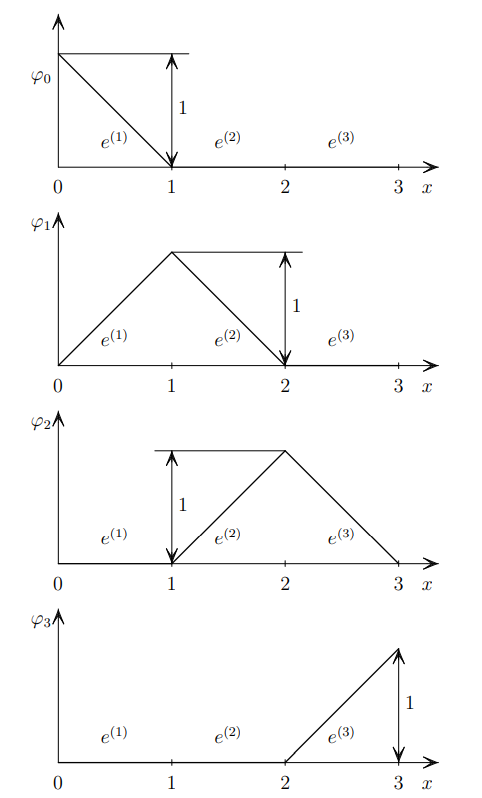
\includegraphics[scale=0.4]{basis_1d}
	\caption{Кусочно-линейные базисные функции на одномерной сетке\label{pic:basis_1d}}
\end{figure}

Для таких функций матрица $A$ в системе \eqref{eq:ritz_linsys} является трехдиагональной. Трехдиагональная она потому, что для некоторого $i$ число $[\varphi_i, \varphi_j]$ не равно нулю только для $j = i-1,~i,~i+1$. Можно проверить, что итоговая трехдиагональная матрица практически совпадает с матрицей, которую дает метод конечных разностей.

\subsection{Кусочно-линейные функции на треугольниках}
Такой подход можно расширить и на треугольники. Пример базисной функции для одного узла приведен на рисунке \ref{pic:p1}.
\begin{figure}[h] \centering
	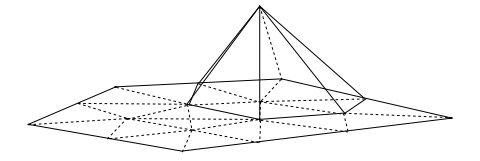
\includegraphics[scale=0.4]{p1}
	\caption{Кусочно-линейная базисная функция на треугольной сетке\label{pic:p1}}
\end{figure}
Такая функция не равна 0 только в ячейках, которые окружают узел, которому она соответствует. В этих треугольниках она ведет себя линейно. Во всех остальных ячейках она нулевая. 

Если рассмотреть некоторый треугольник с вершинами $(x_1,y_1)$, $(x_2,y_2)$, $(x_3,y_3)$ и ввести на нем локальную нумерацию узлов, то базисные функции $\varphi_1$, $\varphi_2$, $\varphi_3$ этих узлов на данном треугольнике имеют вид 
\begin{equation}\label{eq:loc_phi_1}
\varphi_1(x,y) = \frac{(x - x_3)(y_2 - y_3) - (x_2 - x_3)(y - y_3)}{(x_1 - x_3)(y_2 - y_3) - (x_2 - x_3)(y_1 - y_3)}
\end{equation}
\begin{equation}\label{eq:loc_phi_2}
\varphi_2(x,y) = \frac{(x - x_3)(y_1 - y_3) - (x_1 - x_3)(y - y_3)}{(x_2 - x_3)(y_1 - y_3) - (x_1 - x_3)(y_2 - y_3)}
\end{equation}
\begin{equation}\label{eq:loc_phi_3}
\varphi_3(x,y) = \frac{(x - x_1)(y_2 - y_1) - (x_2 - x_1)(y - y_1)}{(x_3 - x_1)(y_2 - y_1) - (x_2 - x_1)(y_3 - y_1)}
\end{equation}

\subsubsection{Особенности сборки матрицы жесткости}
Можно догадаться, что значение $[\varphi_i, \varphi_j]$ не равно 0 только в том случае, если узлы $i$ и $j$ являются вершинами одного треугольника.  
\begin{figure}[h] \centering
	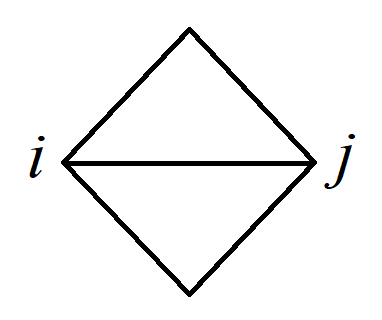
\includegraphics[scale=0.4]{two_cells}
	\caption{Два узла $i$ и $j$, чьи базисные функции одновременно не равны нулю на двух треугольниках\label{pic:two_cells}}
\end{figure}

Заполнение матрицы жесткости $A$ \eqref{eq:ritz_linsys} можно проводить по-разному. Например, можно заполнять матрицу по строкам. Каждая строка соответствует одному узлу. В ходе заполнения строки для $i$-го узла нужно вычислять все ненулевые произведения $[\varphi_i, \varphi_j]$. Для соседних узлов $i$ и $j$ их базисные функции не равны нулю одновременно на двух треугольниках. Таким образом, для вычисления $[\varphi_i, \varphi_j]$ нужно будет обратиться к двум разным треугольникам, чтобы произвести интегрирование. Более того, в ходе заполнения строки для $i$-го узла к каждому из соседних треугольников придется обратиться 2 раза при вычислении функций для разных соседних узлов. Это все приводит к лишним вычислениям.

Поэтому сборку глобальной матрицы жесткости $A$ выполняют по-другому. Запускается цикл по по ячейкам (треугольникам). На каждом треугольнике рассматриваются $\varphi_1,~\varphi_2,~\varphi_3$ (используется локальная для треугольника нумерация узлов). Далее для этих трех функций вычисляются все попарные скалярные произведения, записывающиеся в \textit{локальную} матрицу жесткости. После чего локальная матрица встраивается в глобальную.
%\section{Программная реализация МКЭ с кусочно-линейными функциями на треугольниках}
%Опишем программную реализацию метода с помощью платформы INMOST. 
%\subsection{Хранение данных на сетке}
%Необходимые сеточные данные будем хранить в тегах -- объектах класса \texttt{Tag}. Входными данными являются тензор фильтрации $D$
\section{Практические задания}
Эти упражнения готовят к основной цели -- программированию настоящего МКЭ.
\begin{enumerate}
	\item Освоить готовые функции в \texttt{src/main.cpp}: создание тегов и циклы по сеточным элементам, получение существующих на сетке тегов, вычисление диаметра сетки, подсчет $C$- и $L_2$-норм разности сеточных функций, представленных ячеечными тегами, создание и решение линейных систем;
	\item Имеется некоторая функция $f$. Она приближается на треугольной сетке функцией $f_N$ -- линейной комбинацией кусочно-линейных функций-<<домиков>>, где каждая кусочно-линейная функция соответствует узлу сетки, а коэффициент при ней является значением приближаемой функции $f$ в этом узле, т.е. $f_N = f(x_1)\phi_1(x) + \dots + f(x_N)\varphi_N(x)$, где $x$ -- координаты в двумерном пространстве. Написать функцию, которая считает $||f-f_N||_C,~~||f-f_N||_{L_2}$. Подсказка: при подсчете $L_2$-нормы нужно запустить цикл по ячейкам, и интегралы считать для каждой ячейки. Для интегрирования использовать квадратурную формулу из методичики, стр. 39.
	\item Построить последовательность измельчающихся треугольных сеток в единичном квадрате с помощью Gmsh. Пользуясь результатами предыдущего задания, приблизить на этих сетку функцию $f = sin(\Pi x) * sin(\Pi y)$. Нарисовать графики $C$- и $L_2$-норм ошибки в зависимости от диаметра сетки. На графике оси сделать в логарифмической шкале.
\end{enumerate}
\end{document}